\section{Analog/Digital Converter}

\subsection{AD-Converter System}

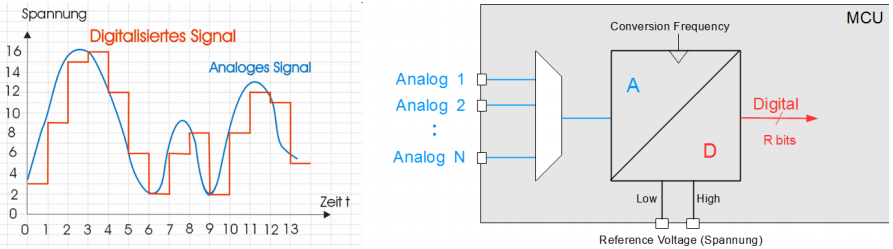
\includegraphics[width=0.5\textwidth]{analog-digital-converter-system.png}

\begin{itemize}
    \item{\textit{
        Many sensor measure values are provided as an analog signal
        (e.g. temperature, pressure, velocity, etc.). For further processing, the
        values are converted into \textbf{R bits (resolution)} wide digital signals.
    }}
    \item{\textit{
        Many MCUs are equipped with an integrated \textbf{A/D-Converter}, that can
        convert multiple analog input voltages from the MCU-Pins with \textbf{timemultiplexing}.
    }}
\end{itemize}

\subsection{Successive Approximation}

\begin{wrapfigure}{l}{0.24\textwidth}
    \centering
    \hspace{-20pt}
    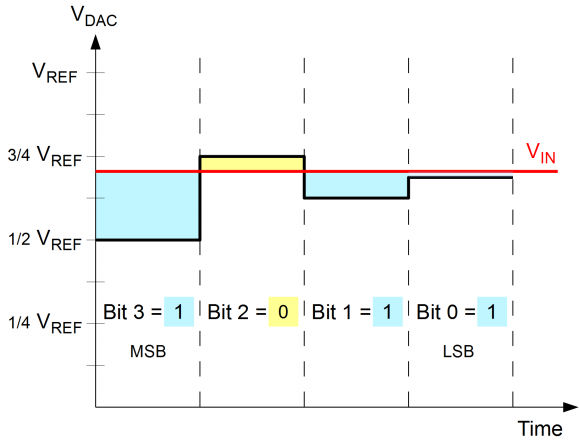
\includegraphics[width=0.24\textwidth]{digital-analog-converter-successvie-approximation.png}
    \hspace{-50pt}
\end{wrapfigure}

\textit{
    The integrated \textbf{A/D}-Converter does comparisions
    step by step, beginning with the MSB.\newline
    Simply its a binary search through comparing.\newline
    The more Bits the generated digital word has,
    the closer the proximity will be.
}

\textit{
    During the conversion, the input voltage is kept
    steady (\textbf{Sample \& Hold}).
}

\subsection{Function Scheme \& Control Register}

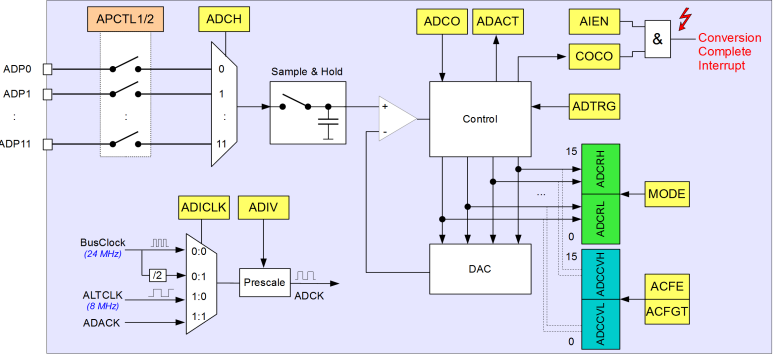
\includegraphics[width=0.5\textwidth]{analog-digital-converter-schema.png}


\begin{tabular}{ll}
    \textbf{ADCO}: 1x, continuous         & \textbf{ADACT}: busy \\
    \textbf{ADTRIG}: ADCSC1 wr, ADHWT pin & \textbf{MODE}: 8, 10, 12bit \\
    \textbf{ACFE}: enable    & \textbf{ACFGT}: less, greater \\
\end{tabular}

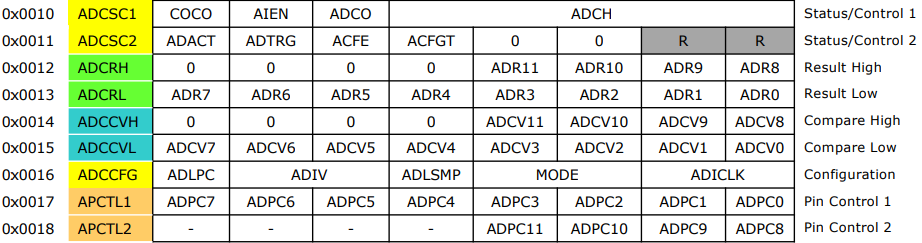
\includegraphics[width=0.5\textwidth]{analog-digital-converter-control-registers.png}

\subsection{Code Sample}

\begin{lstlisting}
#define ADC_RES_8BIT      0
#define ADC_RES_10BIT     2
#define ADC_RES_12BIT     1

// init, using - high speed mode, ADCK = 6 MHz (busclock / 4), enable four line sensor
void adcInit(void)
{
  // max conversion time: 40x ADCK cycles + 5 bus clock cycles
  // 40x 167ns + 5x 42ns = 7.21us
  // long sample time for higher conversion accuracy
  ADCCFG_ADLPC = 0;       // high speed
  ADCCFG_ADLSMP = 1;      // long sample time
  ADCCFG_ADICLK = 0;      // bus clock = 24 MHz

  // create mask for only reading used channels, prevents external noise
  APCTL1 = 0xF0;          // LsL, LsML. LsMR, LsR
  //APCTL1 = (1<<adcLsL) | (1<<adcLsML) | (1<<adcLsMR) |  (1<<adcLsR);

  // valid clock: 0.4 - 4 MHz if ADLPC = 1
  ADCCFG_ADIV = 2;        // 0=/1,  1=/2,  2=/4, 3=/8

  // setup interrupt (compare value - 12bit)
  ADCCV = 0x05;
  // define if trigger on less (0) or greater (1) then recevied value
  ACFGT = 0; //
  ACFE = 1; // enable compare function
  AIEN = 1; // enable interrupt
  // to reset the interrupt flag (COCO), eather write to ADCSC1 or read ADCRL
}

// 12 bit resolution (most of the time to much noise prever 10/8 Bit)
uint16 adcGet12BitValue(AdcChannels ch)
{
    // set resolution (could also be ADC_RES_10BIT or ADC_RES_12BIT)
    ADCCFG_MODE = ADC_RES_12BIT;
    // start new conversion and reset COCO (interrupt flag)
    ADCSC1_ADCH = (uint8)ch;
    // wait until conversion has completed
    while(!ADCSC1_COCO);
    return ADCR;
}
\end{lstlisting}
